% Options for packages loaded elsewhere
\PassOptionsToPackage{unicode}{hyperref}
\PassOptionsToPackage{hyphens}{url}
\PassOptionsToPackage{dvipsnames,svgnames,x11names}{xcolor}
%
\documentclass[
  letterpaper,
  DIV=11,
  numbers=noendperiod,
  oneside]{scrreprt}

\usepackage{amsmath,amssymb}
\usepackage{iftex}
\ifPDFTeX
  \usepackage[T1]{fontenc}
  \usepackage[utf8]{inputenc}
  \usepackage{textcomp} % provide euro and other symbols
\else % if luatex or xetex
  \usepackage{unicode-math}
  \defaultfontfeatures{Scale=MatchLowercase}
  \defaultfontfeatures[\rmfamily]{Ligatures=TeX,Scale=1}
\fi
\usepackage{lmodern}
\ifPDFTeX\else  
    % xetex/luatex font selection
\fi
% Use upquote if available, for straight quotes in verbatim environments
\IfFileExists{upquote.sty}{\usepackage{upquote}}{}
\IfFileExists{microtype.sty}{% use microtype if available
  \usepackage[]{microtype}
  \UseMicrotypeSet[protrusion]{basicmath} % disable protrusion for tt fonts
}{}
\makeatletter
\@ifundefined{KOMAClassName}{% if non-KOMA class
  \IfFileExists{parskip.sty}{%
    \usepackage{parskip}
  }{% else
    \setlength{\parindent}{0pt}
    \setlength{\parskip}{6pt plus 2pt minus 1pt}}
}{% if KOMA class
  \KOMAoptions{parskip=half}}
\makeatother
\usepackage{xcolor}
\usepackage[left=1in,marginparwidth=2.0666666666667in,textwidth=4.1333333333333in,marginparsep=0.3in]{geometry}
\setlength{\emergencystretch}{3em} % prevent overfull lines
\setcounter{secnumdepth}{5}
% Make \paragraph and \subparagraph free-standing
\ifx\paragraph\undefined\else
  \let\oldparagraph\paragraph
  \renewcommand{\paragraph}[1]{\oldparagraph{#1}\mbox{}}
\fi
\ifx\subparagraph\undefined\else
  \let\oldsubparagraph\subparagraph
  \renewcommand{\subparagraph}[1]{\oldsubparagraph{#1}\mbox{}}
\fi

\usepackage{color}
\usepackage{fancyvrb}
\newcommand{\VerbBar}{|}
\newcommand{\VERB}{\Verb[commandchars=\\\{\}]}
\DefineVerbatimEnvironment{Highlighting}{Verbatim}{commandchars=\\\{\}}
% Add ',fontsize=\small' for more characters per line
\usepackage{framed}
\definecolor{shadecolor}{RGB}{241,243,245}
\newenvironment{Shaded}{\begin{snugshade}}{\end{snugshade}}
\newcommand{\AlertTok}[1]{\textcolor[rgb]{0.68,0.00,0.00}{#1}}
\newcommand{\AnnotationTok}[1]{\textcolor[rgb]{0.37,0.37,0.37}{#1}}
\newcommand{\AttributeTok}[1]{\textcolor[rgb]{0.40,0.45,0.13}{#1}}
\newcommand{\BaseNTok}[1]{\textcolor[rgb]{0.68,0.00,0.00}{#1}}
\newcommand{\BuiltInTok}[1]{\textcolor[rgb]{0.00,0.23,0.31}{#1}}
\newcommand{\CharTok}[1]{\textcolor[rgb]{0.13,0.47,0.30}{#1}}
\newcommand{\CommentTok}[1]{\textcolor[rgb]{0.37,0.37,0.37}{#1}}
\newcommand{\CommentVarTok}[1]{\textcolor[rgb]{0.37,0.37,0.37}{\textit{#1}}}
\newcommand{\ConstantTok}[1]{\textcolor[rgb]{0.56,0.35,0.01}{#1}}
\newcommand{\ControlFlowTok}[1]{\textcolor[rgb]{0.00,0.23,0.31}{#1}}
\newcommand{\DataTypeTok}[1]{\textcolor[rgb]{0.68,0.00,0.00}{#1}}
\newcommand{\DecValTok}[1]{\textcolor[rgb]{0.68,0.00,0.00}{#1}}
\newcommand{\DocumentationTok}[1]{\textcolor[rgb]{0.37,0.37,0.37}{\textit{#1}}}
\newcommand{\ErrorTok}[1]{\textcolor[rgb]{0.68,0.00,0.00}{#1}}
\newcommand{\ExtensionTok}[1]{\textcolor[rgb]{0.00,0.23,0.31}{#1}}
\newcommand{\FloatTok}[1]{\textcolor[rgb]{0.68,0.00,0.00}{#1}}
\newcommand{\FunctionTok}[1]{\textcolor[rgb]{0.28,0.35,0.67}{#1}}
\newcommand{\ImportTok}[1]{\textcolor[rgb]{0.00,0.46,0.62}{#1}}
\newcommand{\InformationTok}[1]{\textcolor[rgb]{0.37,0.37,0.37}{#1}}
\newcommand{\KeywordTok}[1]{\textcolor[rgb]{0.00,0.23,0.31}{#1}}
\newcommand{\NormalTok}[1]{\textcolor[rgb]{0.00,0.23,0.31}{#1}}
\newcommand{\OperatorTok}[1]{\textcolor[rgb]{0.37,0.37,0.37}{#1}}
\newcommand{\OtherTok}[1]{\textcolor[rgb]{0.00,0.23,0.31}{#1}}
\newcommand{\PreprocessorTok}[1]{\textcolor[rgb]{0.68,0.00,0.00}{#1}}
\newcommand{\RegionMarkerTok}[1]{\textcolor[rgb]{0.00,0.23,0.31}{#1}}
\newcommand{\SpecialCharTok}[1]{\textcolor[rgb]{0.37,0.37,0.37}{#1}}
\newcommand{\SpecialStringTok}[1]{\textcolor[rgb]{0.13,0.47,0.30}{#1}}
\newcommand{\StringTok}[1]{\textcolor[rgb]{0.13,0.47,0.30}{#1}}
\newcommand{\VariableTok}[1]{\textcolor[rgb]{0.07,0.07,0.07}{#1}}
\newcommand{\VerbatimStringTok}[1]{\textcolor[rgb]{0.13,0.47,0.30}{#1}}
\newcommand{\WarningTok}[1]{\textcolor[rgb]{0.37,0.37,0.37}{\textit{#1}}}

\providecommand{\tightlist}{%
  \setlength{\itemsep}{0pt}\setlength{\parskip}{0pt}}\usepackage{longtable,booktabs,array}
\usepackage{calc} % for calculating minipage widths
% Correct order of tables after \paragraph or \subparagraph
\usepackage{etoolbox}
\makeatletter
\patchcmd\longtable{\par}{\if@noskipsec\mbox{}\fi\par}{}{}
\makeatother
% Allow footnotes in longtable head/foot
\IfFileExists{footnotehyper.sty}{\usepackage{footnotehyper}}{\usepackage{footnote}}
\makesavenoteenv{longtable}
\usepackage{graphicx}
\makeatletter
\def\maxwidth{\ifdim\Gin@nat@width>\linewidth\linewidth\else\Gin@nat@width\fi}
\def\maxheight{\ifdim\Gin@nat@height>\textheight\textheight\else\Gin@nat@height\fi}
\makeatother
% Scale images if necessary, so that they will not overflow the page
% margins by default, and it is still possible to overwrite the defaults
% using explicit options in \includegraphics[width, height, ...]{}
\setkeys{Gin}{width=\maxwidth,height=\maxheight,keepaspectratio}
% Set default figure placement to htbp
\makeatletter
\def\fps@figure{htbp}
\makeatother

\KOMAoption{captions}{tableheading}
\makeatletter
\@ifpackageloaded{tcolorbox}{}{\usepackage[skins,breakable]{tcolorbox}}
\@ifpackageloaded{fontawesome5}{}{\usepackage{fontawesome5}}
\definecolor{quarto-callout-color}{HTML}{909090}
\definecolor{quarto-callout-note-color}{HTML}{0758E5}
\definecolor{quarto-callout-important-color}{HTML}{CC1914}
\definecolor{quarto-callout-warning-color}{HTML}{EB9113}
\definecolor{quarto-callout-tip-color}{HTML}{00A047}
\definecolor{quarto-callout-caution-color}{HTML}{FC5300}
\definecolor{quarto-callout-color-frame}{HTML}{acacac}
\definecolor{quarto-callout-note-color-frame}{HTML}{4582ec}
\definecolor{quarto-callout-important-color-frame}{HTML}{d9534f}
\definecolor{quarto-callout-warning-color-frame}{HTML}{f0ad4e}
\definecolor{quarto-callout-tip-color-frame}{HTML}{02b875}
\definecolor{quarto-callout-caution-color-frame}{HTML}{fd7e14}
\makeatother
\makeatletter
\makeatother
\makeatletter
\@ifpackageloaded{bookmark}{}{\usepackage{bookmark}}
\makeatother
\makeatletter
\@ifpackageloaded{caption}{}{\usepackage{caption}}
\AtBeginDocument{%
\ifdefined\contentsname
  \renewcommand*\contentsname{Table of contents}
\else
  \newcommand\contentsname{Table of contents}
\fi
\ifdefined\listfigurename
  \renewcommand*\listfigurename{List of Figures}
\else
  \newcommand\listfigurename{List of Figures}
\fi
\ifdefined\listtablename
  \renewcommand*\listtablename{List of Tables}
\else
  \newcommand\listtablename{List of Tables}
\fi
\ifdefined\figurename
  \renewcommand*\figurename{Figure}
\else
  \newcommand\figurename{Figure}
\fi
\ifdefined\tablename
  \renewcommand*\tablename{Table}
\else
  \newcommand\tablename{Table}
\fi
}
\@ifpackageloaded{float}{}{\usepackage{float}}
\floatstyle{ruled}
\@ifundefined{c@chapter}{\newfloat{codelisting}{h}{lop}}{\newfloat{codelisting}{h}{lop}[chapter]}
\floatname{codelisting}{Listing}
\newcommand*\listoflistings{\listof{codelisting}{List of Listings}}
\makeatother
\makeatletter
\@ifpackageloaded{caption}{}{\usepackage{caption}}
\@ifpackageloaded{subcaption}{}{\usepackage{subcaption}}
\makeatother
\makeatletter
\@ifpackageloaded{tcolorbox}{}{\usepackage[skins,breakable]{tcolorbox}}
\makeatother
\makeatletter
\@ifundefined{shadecolor}{\definecolor{shadecolor}{rgb}{.97, .97, .97}}
\makeatother
\makeatletter
\makeatother
\makeatletter
\@ifpackageloaded{sidenotes}{}{\usepackage{sidenotes}}
\@ifpackageloaded{marginnote}{}{\usepackage{marginnote}}
\makeatother
\makeatletter
\makeatother
\ifLuaTeX
  \usepackage{selnolig}  % disable illegal ligatures
\fi
\IfFileExists{bookmark.sty}{\usepackage{bookmark}}{\usepackage{hyperref}}
\IfFileExists{xurl.sty}{\usepackage{xurl}}{} % add URL line breaks if available
\urlstyle{same} % disable monospaced font for URLs
\hypersetup{
  pdftitle={Linear Algebra in Data Science},
  pdfauthor={Norman Matloff},
  colorlinks=true,
  linkcolor={blue},
  filecolor={Maroon},
  citecolor={Blue},
  urlcolor={Blue},
  pdfcreator={LaTeX via pandoc}}

\title{Linear Algebra \emph{in} Data Science}
\usepackage{etoolbox}
\makeatletter
\providecommand{\subtitle}[1]{% add subtitle to \maketitle
  \apptocmd{\@title}{\par {\large #1 \par}}{}{}
}
\makeatother
\subtitle{An unconventional approach}
\author{Norman Matloff}
\date{2024-11-27}

\begin{document}
\maketitle
\ifdefined\Shaded\renewenvironment{Shaded}{\begin{tcolorbox}[frame hidden, interior hidden, sharp corners, enhanced, boxrule=0pt, breakable, borderline west={3pt}{0pt}{shadecolor}]}{\end{tcolorbox}}\fi

\renewcommand*\contentsname{Table of contents}
{
\hypersetup{linkcolor=}
\setcounter{tocdepth}{2}
\tableofcontents
}
\bookmarksetup{startatroot}

\hypertarget{preface}{%
\chapter*{Preface}\label{preface}}
\addcontentsline{toc}{chapter}{Preface}

\markboth{Preface}{Preface}

\newpage

Welcome to my magnum opus! :-) I've written a number of books, but
consider this one to be the most important.
{\marginnote{\begin{footnotesize}This work is licensed under Creative
Commons Zero v1.0 Universal\end{footnotesize}}}

\hypertarget{subtlety-in-the-title}{%
\subsection*{Subtlety in the Title}\label{subtlety-in-the-title}}
\addcontentsline{toc}{subsection}{Subtlety in the Title}

Let's start with the title of this book, ``Linear Algebra \emph{in} Data
Science.'' It would be more typical of ``math support for field X''
books to use ``for'' rather than ``in,'' but the use of the latter aims
to emphasize the fact that:

Linear algebra is absolutely fundamental to the Data Science field. For
us data scientists, it is ``our'' branch of math. Mastering this branch,
which is definitely within the reach of all, pays major dividends.

\hypertarget{philosophy}{%
\subsection*{Philosophy}\label{philosophy}}
\addcontentsline{toc}{subsection}{Philosophy}

This is an unconventional linear algebra textbook, doing everything
``backwards.'' The presentation of each concept begins with a problem to
be solved, almost always from Data Science, leading up to a linear
algebra solution. Basically, the math sneaks up on the reader, who
suddenly realizes they've just learned a new general concept!

\hypertarget{who-is-this-book-for}{%
\subsection*{Who is this book for?}\label{who-is-this-book-for}}
\addcontentsline{toc}{subsection}{Who is this book for?}

Of course the book should work well as a course textbook. The
``applications first'' approach should motivate student, and the use of
Quarto enables easy conversion to Powerpoint by instructors.

I hope the book's emphasize on the Why? and How? especially appeals to
do-it-yourselfers, those who engagement in self-study is motivated by
intellectual curiosity rather than a course grade.

\hypertarget{prerequisite-background}{%
\subsection*{Prerequisite background}\label{prerequisite-background}}
\addcontentsline{toc}{subsection}{Prerequisite background}

Basic data science:

\begin{itemize}
\item
  Calculus.
\item
  Some exposure to R is recommended, but the text can be read without
  it.{\marginnote{\begin{footnotesize}For a quick, painless introduction
  to R, see my \href{https://github.com/matloff/fasteR}{fasteR}
  tutorial, say the first 8 lessons.\end{footnotesize}}}
\item
  Basics of random variables, expected value and variance.
\end{itemize}

\bookmarksetup{startatroot}

\hypertarget{matrix-multiplication}{%
\chapter{Matrix Multiplication}\label{matrix-multiplication}}

\newpage{}

\hypertarget{a-random-walk-model}{%
\section{A Random Walk Model}\label{a-random-walk-model}}

Let's consider a \emph{random walk} on \{1,2,3,4,5\} in the number line.
Time is numbered 1,2,3,\ldots{} Our current position is termed our
\emph{state}. The notation X\textsubscript{k} = i means that at time k
we are in state/position i.

Our rule will be that at any time k, we flip a coin. If we are currently
at position i, we move to either i+1 or i-1, depending on whether the
coin landed heads or tails. The exceptions are k = 1 and k = 5, in which
case we stay put if tails or move to the adjacent position if heads.

We can summarize the probabilities with a \emph{matrix}, a
two-dimensional array:

\[
P_1 =
\left (
\begin{array}{rrrrr}
0.5 & 0.5 & 0 & 0 & 0\\
0.5 & 0 & 0.5 & 0 & 0\\
0 & 0.5 & 0 & 0.5 & 0\\
0 & 0 & 0.5 & 0 & 0.5\\
0 & 0 & 0 & 0.5 & 0.5 \\
\end{array}
\right )
\]

For instance, look at Row 2. There are 0.5 values in Columns 1 and 3,
meaning there is a 0.5 chance of a move 2 \(\rightarrow\) 1, and a 0.5
chance of a move 2 \(\rightarrow\) 3.
{\marginnote{\begin{footnotesize}Note that each row in a transition
matrix must sum to 1. After, from state i we must go
\emph{somewhere}.\end{footnotesize}}}

We use a subscript 1 here in \(P_1\), meaning ``one step.'' We go from,
say, state 2 to state 1 in one step with probability 0.5. \(P_1\) is
called the \emph{one-step transition matrix} (or simply the
\emph{transition matrix}) for this process.

What about the two-step transition matrix \(P_2\)? From state 3, we
could go to state 1 in two steps, by two tails flips of the coin. The
probability of that is \(0.5^2 = 0.25\). So the row 3, column 1 element
in \(P_2\) is 0.25. On the other hand, if from state 3 we flip tails
then heads, or heads then tails, we are back to state 3. So, the row 3,
column 3 element in \(P_2\) is 0.25 + 0.25 = 0.5.

The reader should verify the correctness here:

\[
P_2 =
\left (
\begin{array}{rrrrr}
0.5 & 0.25 & 0.25 & 0 & 0\\
0.25 & 0.5 & 0 & 0.25 & 0\\
0.25 & 0 & 0.5 & 0 & 0.25\\
0 & 0.25 & 0 & 0.5 & 0.25\\
0 & 0 & 0.25 & 0.25 & 0.5 \\
\end{array}
\right )
\]

Well, finding two-step transition probabilities would be tedious in
general, but it turns out that is a wonderful shortcut: Matrix
multiplication. We will cover this in the next section, but first a
couple of preliminaries.

The above random walk is a \emph{Markov chain}. The Markov Property says
that the system ``has no jemory.'' If say we land at position 2, we will
go to 1 or 3 with probability 1/2 \emph{no matter what the previous
history of the system was}; it doesn't matter \emph{how} we got to state
3. That in turn comes from the independence of the successive coin
flips.

\textbf{Notation:} Individual elements of a matrix are usually written
with double subscripts. For instance, a25 will mean the row 2, column 5
element of the matrix A.

\hypertarget{matrix-multiplication-1}{%
\section{Matrix Multiplication}\label{matrix-multiplication-1}}

This is the most fundamental operation in linear algebra. It is defined
as follows:

Given matrix A of k rows and m columns and matrix B of m rows and r
columns, the product C = AB is an kxm matrix, whose row i, column j
element is

\[
a_{i1} b_{i1} +
a_{i2} b_{i1} + ... +
a_{m1} b_{m1} 
\]

This is the ``dot product'' of row i of A and column j of B: Find the
products of the paired elements in the two vectors, then sum.

{\marginnote{\begin{footnotesize}Be sure to remember that the number of
rows of B must match the number of columns of A. In this case, we say
thst the matrices are \emph{conformable}.\end{footnotesize}}}

For example, set

\[
A = \left (
\begin{array}{rr}
5 & 2 & 6 \\
1 & 1 & 8 \\
\end{array}
\right )
\]

and

\[
B = \left (
\begin{array}{rrr}
5 & -1 \\
1 & 0 \\
0 & 8 \\
\end{array}
\right )
\]

Let's find the row 2, column 2 element of C = AB. Again, that means
taking the dot product of row 2 of A and column 2 of B, which we've
highlighted below.

\[
A = \left (
\begin{array}{rr}
5 & 2 & 6 \\
\color{red}{1} & \color{red}{1} & \color{red}{1} \\
\end{array}
\right )
\]

and

\[
B = \left (
\begin{array}{rrr}
5 & \color{red}{-1} \\
1 & \color{red}{0} \\
0 & \color{red}{8} \\
\end{array}
\right )
\]

The value in question is then

1 (-1) + 1 (0) + 1 (8) = 7

Let's check it, with R:

{\marginnote{\begin{footnotesize}.The \textbf{rbind} and \textbf{cbind}
functions (``row bind'' and ``column bind'') are very handy tools for
creating matrices.\end{footnotesize}}}

\begin{Shaded}
\begin{Highlighting}[]
\NormalTok{a }\OtherTok{\textless{}{-}} \FunctionTok{rbind}\NormalTok{(}\FunctionTok{c}\NormalTok{(}\DecValTok{5}\NormalTok{,}\DecValTok{2}\NormalTok{,}\DecValTok{6}\NormalTok{),}\FunctionTok{c}\NormalTok{(}\DecValTok{1}\NormalTok{,}\DecValTok{1}\NormalTok{,}\DecValTok{1}\NormalTok{))}
\NormalTok{b }\OtherTok{\textless{}{-}} \FunctionTok{cbind}\NormalTok{(}\FunctionTok{c}\NormalTok{(}\DecValTok{5}\NormalTok{,}\DecValTok{1}\NormalTok{,}\DecValTok{0}\NormalTok{),}\FunctionTok{c}\NormalTok{(}\SpecialCharTok{{-}}\DecValTok{1}\NormalTok{,}\DecValTok{0}\NormalTok{,}\DecValTok{8}\NormalTok{))}
\NormalTok{a }\SpecialCharTok{\%*\%}\NormalTok{ b}
\end{Highlighting}
\end{Shaded}

\begin{verbatim}
     [,1] [,2]
[1,]   27   43
[2,]    6    7
\end{verbatim}

The reader should make sure to check the other elements by hand.

\hypertarget{vectors}{%
\section{Vectors}\label{vectors}}

A matrix that has only one row or only one column is called a
\emph{vector}. Depending on which of those two shapes it has, we may
refer to it as a \emph{row vector} or \emph{column vector}. Usually we
will simply say ``vector,'' in which case it will be meant as a column
vector.

\hypertarget{sec-introMCs}{%
\section{Application to Markov Chain Transition
Matrices}\label{sec-introMCs}}

Now let's return to the question of how to easily compute \(P_2\), the
two-step transition matrix. It turns out that:

Let P denote the transition matrix of a (finite-state) Markov chain. The
k-step transition matrix is \(P^k\).

At first, this may seem amazingly fortuitous, but it makes sense in
light of the ``and/or'' nature of the probability computations involved.
Recall our computation for the row 1, column 2 element of \(P_2\) above.
From state 1, we could either stay at 1 for one flip, then move to 2 on
the second flip, or we could go to 2 then return to 1. Each of these has
probability 0.5, so the total probability is

\[
(0.5)(0.5) + (0.5)(0.5)
\]

But this is exactly the form of our ``dot product'' computation in the
definition of matrix multiplication,

\[
a_{i1} b_{i1} +
a_{i2} b_{i1} + ... +
a_{m1} b_{m1} 
\]

Statisticians and computer scientists like to look at the
\emph{asymptotic} behavior of systems. Let's see where we might be after
say, 6 steps:{\marginnote{\begin{footnotesize}The \emph{identity matrix}
I of size n is the nxn matrix with 1s on the diagonal and 0s elsewhere.
IB = B and AI = A for any conformable A and B.\end{footnotesize}}}

\begin{Shaded}
\begin{Highlighting}[]
\NormalTok{matpow }\OtherTok{\textless{}{-}} \ControlFlowTok{function}\NormalTok{(m,k) \{}
\NormalTok{   nr }\OtherTok{\textless{}{-}} \FunctionTok{nrow}\NormalTok{(m)}
\NormalTok{   tmp }\OtherTok{\textless{}{-}} \FunctionTok{diag}\NormalTok{(nr)  }\CommentTok{\# identity matrix}
   \ControlFlowTok{for}\NormalTok{ (i }\ControlFlowTok{in} \DecValTok{1}\SpecialCharTok{:}\NormalTok{k) tmp }\OtherTok{\textless{}{-}}\NormalTok{ tmp }\SpecialCharTok{\%*\%}\NormalTok{ m}
\NormalTok{   tmp}
\NormalTok{\}}

\NormalTok{p1 }\OtherTok{\textless{}{-}} \FunctionTok{rbind}\NormalTok{(}\FunctionTok{c}\NormalTok{(}\FloatTok{0.5}\NormalTok{,}\FloatTok{0.5}\NormalTok{,}\DecValTok{0}\NormalTok{,}\DecValTok{0}\NormalTok{,}\DecValTok{0}\NormalTok{), }\FunctionTok{c}\NormalTok{(}\FloatTok{0.5}\NormalTok{,}\DecValTok{0}\NormalTok{,}\FloatTok{0.5}\NormalTok{,}\DecValTok{0}\NormalTok{,}\DecValTok{0}\NormalTok{), }\FunctionTok{c}\NormalTok{(}\DecValTok{0}\NormalTok{,}\FloatTok{0.5}\NormalTok{,}\DecValTok{0}\NormalTok{,}\FloatTok{0.5}\NormalTok{,}\DecValTok{0}\NormalTok{), }
   \FunctionTok{c}\NormalTok{(}\DecValTok{0}\NormalTok{,}\DecValTok{0}\NormalTok{,}\FloatTok{0.5}\NormalTok{,}\DecValTok{0}\NormalTok{,}\FloatTok{0.5}\NormalTok{), }\FunctionTok{c}\NormalTok{(}\DecValTok{0}\NormalTok{,}\DecValTok{0}\NormalTok{,}\DecValTok{0}\NormalTok{,}\FloatTok{0.5}\NormalTok{,}\FloatTok{0.5}\NormalTok{))}
\FunctionTok{matpow}\NormalTok{(}\FunctionTok{t}\NormalTok{(p1),}\DecValTok{6}\NormalTok{) }\CommentTok{\# R uses t() for transpose}
\end{Highlighting}
\end{Shaded}

\begin{verbatim}
         [,1]     [,2]     [,3]     [,4]     [,5]
[1,] 0.312500 0.234375 0.234375 0.109375 0.109375
[2,] 0.234375 0.312500 0.109375 0.234375 0.109375
[3,] 0.234375 0.109375 0.312500 0.109375 0.234375
[4,] 0.109375 0.234375 0.109375 0.312500 0.234375
[5,] 0.109375 0.109375 0.234375 0.234375 0.312500
\end{verbatim}

So for instance if we start at position 2, there is about an 11\% chance
that we will be at position 3 at time 6. What about time 25?

\begin{Shaded}
\begin{Highlighting}[]
\FunctionTok{matpow}\NormalTok{(}\FunctionTok{t}\NormalTok{(p1),}\DecValTok{25}\NormalTok{)}
\end{Highlighting}
\end{Shaded}

\begin{verbatim}
          [,1]      [,2]      [,3]      [,4]      [,5]
[1,] 0.2016179 0.2016179 0.1993820 0.1993820 0.1980001
[2,] 0.2016179 0.1993820 0.2016179 0.1980001 0.1993820
[3,] 0.1993820 0.2016179 0.1980001 0.2016179 0.1993820
[4,] 0.1993820 0.1980001 0.2016179 0.1993820 0.2016179
[5,] 0.1980001 0.1993820 0.1993820 0.2016179 0.2016179
\end{verbatim}

So, no matter which state we start in, at time 25 we are about 20\%
likely to be at any of the states. In fact, as time n goes to infinity,
this probability vector becomes exactly (0.20,0.20,0.20,0.20,0.20), as
we will see in the next chapter..

❄️ \textbf{Your Turn:} The long-run probabilities here turned out to be
uniform, with value 0.20 for all five states. In fact, that is usually
not the case. Make a small change to \(P_1\) -- remember to keep the row
sums to 1 -- and compute a high power to check whether the long-run
distribution seems nonuniform.

❄️ \textbf{Your Turn:} Not every Markov chain, even ones with finitely
many states, have long-run distributions. Some chains have
\emph{periodic} states. It may be, for instance, that after leaving
state \(i\), once can return only after an even number of hops. Modify
our example chain here so that states 1 and 5 (and all the others) have
that property. Then compute \(P^n\) for various large values of \(n\)
and observe oscillatory behavior, rather than long-run convergence.

❄️ \textbf{Your Turn:} Consider the following model of a discrete-time,
single-server queue:

\begin{itemize}
\item
  Model parameters are p (probability of job completion), q (probability
  of new job arriving) and m (size of the buffer).
\item
  Jobs arrive, are served (possibly after queuing) and leave.
\item
  Only one job can be in service at a time.
\item
  At each time epoch:

  \begin{itemize}
  \item
    The job currently in service, if any, will complete with probability
    p.
  \item
    Slightly after a possible job completion, a job in the queue, if
    any, will start service.
  \end{itemize}

  a Slightly after that, anew job will arrive with probability q. If the
  queue is empty, this job starts service. If not, and if the queue is
  not full, it will join the queue. Otherwise, the job is discarded.
\item
  The system is memoryless.
\item
  The current state is the number of jobs in the system, taking on the
  values 0,1,2,..,m+1; that last state means m jobs in the queue and 1
  in service.
\end{itemize}

For instance, say p = 0.4, q = 0.2, m = 5, Suppose the current state is
3, so there is a job in service and two jobs in the queue. Our next
state will be 2 with probability (0.4) (0.8); it will be 3 with
probability (0.4) (0.2), and so on.

Analyze this system for the case given above.` Find the approximate
long-run distribution, and also the proportion of jobs that get
discarded.

\hypertarget{network-graph-models}{%
\section{Network Graph Models}\label{network-graph-models}}

There has always been lots of analyses of ``Who is connected to who,''
but activity soared after the advent of Facebook and the film, \emph{A
Social Network.} See for instance \emph{Statistical Analysis of Network
Data with R} by Eric Kolaczy and Gábor Csárdi. As the authors say,

The oft-repeated statement that ``we live in a connected world'' perhaps
best captures, in its simplicity\ldots From on-line social networks like
Facebook to the World Wide Web and the Internet itself, we are
surrounded by examples of ways in which we interact with each other.
Similarly, we are connected as well at the level of various human
institutions (e.g., governments), processes (e.g., economies), and
infrastructures (e.g., the global airline network). And, of course,
humans are surely not unique in being members of various complex,
inter-connected systems. Looking at the natural world around us, we see
a wealth of examples of such systems, from entire eco-systems, to
biological food webs, to collections of inter-acting genes or
communicating neurons.

And of course, at the center of it all is a matrix! Here is why:

Let's consider the famous Karate Club dataset:

{\marginnote{\begin{footnotesize}\end{footnotesize}}}

\begin{Shaded}
\begin{Highlighting}[]
\CommentTok{\# remotes::install\_github("schochastics/networkdata") }
\FunctionTok{library}\NormalTok{(networkdata)}
\FunctionTok{data}\NormalTok{(karate)}
\FunctionTok{library}\NormalTok{(igraph)}
\FunctionTok{plot}\NormalTok{(karate)}
\end{Highlighting}
\end{Shaded}

\begin{figure}[H]

{\centering 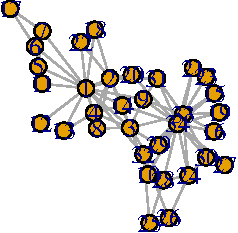
\includegraphics{Ch1_files/figure-pdf/unnamed-chunk-5-1.pdf}

}

\end{figure}

There is a link between node 13 and node 4, meaning that club members 13
and 4 are friends.{\marginnote{\begin{footnotesize}This graph is
\emph{undirected}, as friendship is mutual. Many graphs are
\emph{directed}, but we will assume undirected here.\end{footnotesize}}}

Specifically, the \emph{adjacency matrix} has row i, column j element as
1 or 0, according to whether a link exists between nodes i and j.

\begin{Shaded}
\begin{Highlighting}[]
\NormalTok{adjK }\OtherTok{\textless{}{-}} \FunctionTok{as\_adjacency\_matrix}\NormalTok{(karate)}
\NormalTok{adjK}
\end{Highlighting}
\end{Shaded}

\begin{verbatim}
34 x 34 sparse Matrix of class "dgCMatrix"
                                                                         
 [1,] . 1 1 1 1 1 1 1 1 . 1 1 1 1 . . . 1 . 1 . 1 . . . . . . . . . 1 . .
 [2,] 1 . 1 1 . . . 1 . . . . . 1 . . . 1 . 1 . 1 . . . . . . . . 1 . . .
 [3,] 1 1 . 1 . . . 1 1 1 . . . 1 . . . . . . . . . . . . . 1 1 . . . 1 .
 [4,] 1 1 1 . . . . 1 . . . . 1 1 . . . . . . . . . . . . . . . . . . . .
 [5,] 1 . . . . . 1 . . . 1 . . . . . . . . . . . . . . . . . . . . . . .
 [6,] 1 . . . . . 1 . . . 1 . . . . . 1 . . . . . . . . . . . . . . . . .
 [7,] 1 . . . 1 1 . . . . . . . . . . 1 . . . . . . . . . . . . . . . . .
 [8,] 1 1 1 1 . . . . . . . . . . . . . . . . . . . . . . . . . . . . . .
 [9,] 1 . 1 . . . . . . . . . . . . . . . . . . . . . . . . . . . 1 . 1 1
[10,] . . 1 . . . . . . . . . . . . . . . . . . . . . . . . . . . . . . 1
[11,] 1 . . . 1 1 . . . . . . . . . . . . . . . . . . . . . . . . . . . .
[12,] 1 . . . . . . . . . . . . . . . . . . . . . . . . . . . . . . . . .
[13,] 1 . . 1 . . . . . . . . . . . . . . . . . . . . . . . . . . . . . .
[14,] 1 1 1 1 . . . . . . . . . . . . . . . . . . . . . . . . . . . . . 1
[15,] . . . . . . . . . . . . . . . . . . . . . . . . . . . . . . . . 1 1
[16,] . . . . . . . . . . . . . . . . . . . . . . . . . . . . . . . . 1 1
[17,] . . . . . 1 1 . . . . . . . . . . . . . . . . . . . . . . . . . . .
[18,] 1 1 . . . . . . . . . . . . . . . . . . . . . . . . . . . . . . . .
[19,] . . . . . . . . . . . . . . . . . . . . . . . . . . . . . . . . 1 1
[20,] 1 1 . . . . . . . . . . . . . . . . . . . . . . . . . . . . . . . 1
[21,] . . . . . . . . . . . . . . . . . . . . . . . . . . . . . . . . 1 1
[22,] 1 1 . . . . . . . . . . . . . . . . . . . . . . . . . . . . . . . .
[23,] . . . . . . . . . . . . . . . . . . . . . . . . . . . . . . . . 1 1
[24,] . . . . . . . . . . . . . . . . . . . . . . . . . 1 . 1 . 1 . . 1 1
[25,] . . . . . . . . . . . . . . . . . . . . . . . . . 1 . 1 . . . 1 . .
[26,] . . . . . . . . . . . . . . . . . . . . . . . 1 1 . . . . . . 1 . .
[27,] . . . . . . . . . . . . . . . . . . . . . . . . . . . . . 1 . . . 1
[28,] . . 1 . . . . . . . . . . . . . . . . . . . . 1 1 . . . . . . . . 1
[29,] . . 1 . . . . . . . . . . . . . . . . . . . . . . . . . . . . 1 . 1
[30,] . . . . . . . . . . . . . . . . . . . . . . . 1 . . 1 . . . . . 1 1
[31,] . 1 . . . . . . 1 . . . . . . . . . . . . . . . . . . . . . . . 1 1
[32,] 1 . . . . . . . . . . . . . . . . . . . . . . . 1 1 . . 1 . . . 1 1
[33,] . . 1 . . . . . 1 . . . . . 1 1 . . 1 . 1 . 1 1 . . . . . 1 1 1 . 1
[34,] . . . . . . . . 1 1 . . . 1 1 1 . . 1 1 1 . 1 1 . . 1 1 1 1 1 1 1 .
\end{verbatim}

\begin{Shaded}
\begin{Highlighting}[]
\NormalTok{adjK[}\DecValTok{13}\NormalTok{,}\DecValTok{4}\NormalTok{]}
\end{Highlighting}
\end{Shaded}

\begin{verbatim}
[1] 1
\end{verbatim}

Accordingly, row 13, column 4 does have a 1 entry.

As is the case with Markov transition matrices, powers of an adjacency
matrix can yield valuable information. In the Markov case,
multiplication gives us sums of paired products, computing
probabilities. What about the network graph case?

Here products are of the form 0x0, 0x1, 1x0 or 1x1. If there is a
nonzero entry m in row i, column j of the square of the adjacency
matrix, that means there were m 1x1 products in that sum, which would
correspond to m paths. Let's look into this.

\begin{Shaded}
\begin{Highlighting}[]
\NormalTok{adjK2 }\OtherTok{\textless{}{-}}\NormalTok{ adjK }\SpecialCharTok{\%*\%}\NormalTok{ adjK}
\end{Highlighting}
\end{Shaded}

We see that \textbf{adjK2{[}11,1{]}} is 2. Inspection of \textbf{adjK}
shows that its row 11, columns 6 and 7 are 1s, and that rows 6 and 7,
column 1 are 1s as well. So there are indeed two two-hop paths from node
11 to node 1, specifically \(11 \rightarrow 6 \rightarrow 1\) and \$
\(11 \rightarrow 7 \rightarrow 1\).

Actually, what is typically of interest is \emph{connectivity} rather
than number of paths. For any given pair of nodes, is there a multihop
path between them? Or does the graph break down to several ``islands''
of connected nodes?

Again consider the karate club data.

\begin{Shaded}
\begin{Highlighting}[]
\NormalTok{u }\OtherTok{\textless{}{-}} \FunctionTok{matpow}\NormalTok{(adjK,}\DecValTok{33}\NormalTok{)}
\FunctionTok{sum}\NormalTok{(u }\SpecialCharTok{==} \DecValTok{0}\NormalTok{)}
\end{Highlighting}
\end{Shaded}

\begin{verbatim}
[1] 0
\end{verbatim}

So, in this graph, no pair of nodes has 0 paths between them. The graph
is connected.

Making this kind of analysis fully correct requires paying attention to
things such as cycles. The details are beyond the scope of this book.

\hypertarget{matrix-algebra}{%
\section{Matrix Algebra}\label{matrix-algebra}}

\hypertarget{other-basic-operations}{%
\subsection{Other Basic operations}\label{other-basic-operations}}

Matrix multiplication may seem odd at first, but other operations are
straightforward.

\textbf{Addition:} We just add corresponding elements. For instance,

\[
A = \left (
\begin{array}{rr}
5 & 2 & 6 \\
1 & 2.6 & -1.2 \\
\end{array}
\right )
\]

\[
B = \left (
\begin{array}{rr}
0 & 20 & 6 \\
3 & 5.8 & 1 \\
\end{array}
\right )
\]

\[
A+B = \left (
\begin{array}{rr}
5 & 22 & 12 \\
4 & 8.4 & -0.2 \\
\end{array}
\right )
\]

We do have to make sure the addends match in terms of numbers of rows
and columns, 2 and 3 in the example here.

\textbf{Scalar multiplication:} Again, this is simply elementwise. E.g.
with A as above,

\[
1.5 A = \left (
\begin{array}{rr}
7.5 & 3 & 9 \\
1.5 & 3.9 & -1.8 \\
\end{array}
\right )
\]

\textbf{Distributive property:}

For matrices A, B and C of suitable conformability (A and B match in
numbers of rows and columns, and their common number of columns matches
the number of rows in C), we have

(A+B) C = AC + BC

\hypertarget{matrix-transpose}{%
\subsection{Matrix transpose}\label{matrix-transpose}}

This is a very simple but very important operation: We merely exchange
rows and columns of the given matrix. For instance, with A as above, its
transpose (signified with ``'''), is

\[
A' = \left (
\begin{array}{rr}
5 & 1 \\
2 & 2.6 \\
6 & -1.2 \\
\end{array}
\right )
\]

It can be shown that if A and B are conformable, then

(AB)' = B'A'

For some matrices C, we have C' = C. C is then termed \emph{symmetric}.

We will often write a row vector in the form (a,b,c,\ldots). So (5,1,88)
means the 1x3 matrix with those elements. If we wish this to be a column
vector, we use transpose, so that for instance (5,1,88)' means a 3x1
matrix.

\hypertarget{partitioned-matrices-an-invaluable-visualization-tool}{%
\subsection{Partitioned matrices: an invaluable visualization
tool}\label{partitioned-matrices-an-invaluable-visualization-tool}}

Here, ``visualization'' is not a reference to graphics but rather to
highlighting certain submatrices.

Consider a matrix-vector product Mv. Of course, that means that v is a
column vector whose length is equal to the number of columns of M. If M
is of size rxs, then v is sx1.

Let's denote column j of M by Cj. Then we will see later in this chapter
that

\[
Mv = 
v_1 C_{1} +
v_2 C_{2} + ... +
v_s C_{s}  
\]

For instance, take

\[
A = \left (
\begin{array}{rr}
5 & 2 & 6 \\
1 & 2.6 & -1.2 \\
\end{array}
\right )
\]

and

\[
v = \left (
\begin{array}{rrr}
10 \\
2 \\
1 \\
\end{array}
\right )
\]

The reader should check that

\[
10 \left (
\begin{array}{rr}
5 \\
1 \\
\end{array}
\right )
+
2 \left (
\begin{array}{rr}
2 \\
2.6 \\
\end{array}
\right )
+
1 \left (
\begin{array}{rr}
6 \\
-1.2 \\
\end{array}
\right )
= Av
\]

where the latter is

\[
\left (
\begin{array}{rr}
60 \\
14  \\
\end{array}
\right )
\]

Note that the above expression,

\[
10 \left (
\begin{array}{rr}
5 \\
1 \\
\end{array}
\right )
+
2 \left (
\begin{array}{rr}
2 \\
2.6 \\
\end{array}
\right )
+
1 \left (
\begin{array}{rr}
6 \\
-1.2 \\
\end{array}
\right ),
\]

is a sum of scalar products of vectors, which is called a \emph{linear
combination} of those vectors. In other words, we have that:

The product of a matrix and a column vector is equal to a linear
combination of the columns of the matrix.

Similarly,

The product of a row vector and a matrix is equal to a linear
combination of the rows of the matrix.

❄️ \textbf{Your Turn:} Using the same matrix A and the same vector v as
above, verify that v'A is indeed a linear combination of the rows of A
as described.

To further illustrate partitioned matrices, write the above matrix \(A\)
as

\[
A = 
\left (
\begin{array}{r}
A_{11} & A_{21} \\
\end{array}
\right )
\]

where

\[
A_{11} = 
 \left (
 \begin{array}{rr}
 5 & 2 \\
 1 & 2.6 \\
 \end{array}
 \right )
\]

and

\[
A_{12} = 
 \left (
 \begin{array}{rr}
 6 \\
 -1.2 \\
 \end{array}
 \right )
\]

Symbolically, \(A\) now looks like a 1x2 matrix. Similarly, writing

\[
v = 
 \left (
 \begin{array}{rrr}
 v_{11} \\
 v_{21} \\
 \end{array}
 \right )
\]

where

\[
 v_{11} = 
 \left (
 \begin{array}{rr}
 10 \\
 2 \\
 \end{array}
 \right )
 \]

and \(v_{21} = 1\) (a 1x1 matrix), \(v\) looks to be 2x1.

So, again pretending, treat the product \(Av\) as the multiplication of
a 1x2 ``matrix'' and 2x1 ``vector'', yielding a 1x1 result,

\[
A_{11} v_{11} + A_{12} v_{21}
\]

But all that pretending actually does give the correct answer!

\[
A_{11} v_{11} + A_{12} v_{21} =
 \left (
 \begin{array}{rr}
 5 & 2 \\
 1 & 2.6 \\
 \end{array}
 \right ) 
 \left (
 \begin{array}{rr}
 10 \\
 2 \\
 \end{array}
 \right )
+
 \left (
 \begin{array}{rr}
 6 \\
 -1.2 \\
 \end{array}
 \right )
1 
=
 \left (
 \begin{array}{rr}
 60 \\
 14 \\
 \end{array}
 \right )
\]

\bookmarksetup{startatroot}

\hypertarget{a-further-look-at-markov-chains}{%
\chapter{A Further Look at Markov
Chains}\label{a-further-look-at-markov-chains}}

Suppose \(X_0\), our state at time 0, is random. Let \(f\) denote its
distribution, i.e.~its list of probabilities: \(f_i = P(X_0 = i)\), i =
1,\ldots,k, where k is the number of states in the chain. What about
\(X_1\), the state at time 1? Let's find an expression for \(g\), the
distribution of \(X_1\).{\marginnote{\begin{footnotesize}This section
will be longer than previous ones, but will bring together many of the
concepts. The reader's patience here will be an investment paying great
dividends in the sequel.\end{footnotesize}}}

\[
g_j = P(X_1 = j)
= \sum_{i=1}^k P(X_0 = i) P(X_1 = j | X_0 = i)
= \sum_{i=1}^k f_i a_{ij}
\]

where \(a_{ij}\) is the row i, column j element of the chain's
transition matrix \(P\).

For example, consider \(g_5\). How could we be at state 5 at time 1? We
could start in state 1, probability \(f_1\), then move to state 5,
probability \(a_{15}\), for a total probability of \(f_1 a_{15}\). Or,
we could start in state 2, probability \(f_2\), then move to state 5,
probability \(a_{25}\), for a total probability of \(f_2 a_{25}\). And
so on.

So,

\[
g_j = \sum_{i=1}^k f_i a_{ij}
\]

Putting this is more explicit matrix terms,

\[
g = \left (
\begin{array}{rrrr}
g_1 \\
g_2 \\
... \\
g_k \\
\end{array}
\right )
=
\left (
\begin{array}{rr}
f_1 a_{11} + f_2 a_{21} + ... + f_k a_{k1} \\
f_1 a_{12} + f_2 a_{22} + ... + f_k a_{k2} \\
... \\
f_1 a_{1k} + f_2 a_{2k} + ... + f_k a_{kk} \\
\end{array}
\right )
\]

That last expression is

\[
f'P
\]

so we have the nice compact relation for the distribution of \(X_1\) in
terms of the distribution of \(X_0\).{\marginnote{\begin{footnotesize}By
the way, it won't be used here, but just for practice, note that the
right-hand side, Pf, here is a linear combination of the columns of P,
from our above material on partitioning.\end{footnotesize}}}

\[
g' = f'P
\]

And setting h to the distribution of \(X_2\), the same reasoning gives
us

\[
h' = g'P 
\]

Then since \(g' = f'P\), we have {\marginnote{\begin{footnotesize}Note
that we used the Markov property, ``memorylessness.'' Once we reach time
1, ``time starts over,'' regradless of the previous history,
i.e.~regardless of where we were at time 0.\end{footnotesize}}}

\[
h' = f'P^2 
\]

and so on. Iterating, we obtain

\[
d_j' = d_0' P^j 
\]

where \(d_i\) is the distribution of \(X_i\).

Similarly,

\[
d_j' = d_{j-1}' P
\]

For convenience, let's take transposes:{[}Recall that \((AB)' = B'A'\).

\[
d_j = P' d_{j-1}
\]

Now suppose our chain as a long-run distribution, as in
\{Section~\ref{sec-introMCs}\}. Let's call that distribution \(\nu\). By
lettting \(j \rightarrow \infty\) above, we have

\[
\nu = P' \nu
\]

Since P is known, this provides us with a way to compute \(\nu\). Yes,
finding a high power of P would do this too, but that would involve a
lot of computation, and even then it would not yield the exact answer.
We will return to this in the next chapter.

\bookmarksetup{startatroot}

\hypertarget{matrix-inverse}{%
\chapter{Matrix Inverse}\label{matrix-inverse}}

\newpage{}

This is a fundamental operation in linear algebra (though ironically,
related quantities are often used instead).

\hypertarget{example}{%
\section{Example}\label{example}}

At the end of the last chapter, we found that for a Markov chain with
transition matrix P and stationary distribution \(\nu\),

\[
\nu = P' \nu
\]

This suggests a method for computing \(\nu\), by solving the above
equation.{\marginnote{\begin{footnotesize}\end{footnotesize}}}

Rewrite it using the identity
matrix:{\marginnote{\begin{footnotesize}Recall that for any square
matrix C and identity matrix I of the same size,
\(IC = CI = C\).\end{footnotesize}}}

\[
(I - P') \nu = 0
\]

For the random walk chain in Chapter 1, we
had{\marginnote{\begin{footnotesize}In that particular model, P' = P,
but for most chains this is not the case.\end{footnotesize}}}

\[
P =
\left (
\begin{array}{rrrrr}
0.5 & 0.5 & 0 & 0 & 0\\
0.5 & 0 & 0.5 & 0 & 0\\
0 & 0.5 & 0 & 0.5 & 0\\
0 & 0 & 0.5 & 0 & 0.5\\
0 & 0 & 0 & 0.5 & 0.5 \\
\end{array}
\right )
\]

With \(\nu = (\nu_1,\nu_2,\nu_3,\nu_4,\nu_5)'\), the equation to be
solved, \((I-P') \nu = \nu\), is

\[
\left (
\begin{array}{rrrrr}
0.5 & -0.5 & 0 & 0 & 0 \\
-0.5 & 1 & -0.5 & 0 & 0 \\
0 & -0.5 & 1 & -0.5 & 0 \\
0 & 0 & -0.5 & 1 & -0.5 \\
0 & 0 & 0 & -0.5 & 0.5 \\
\end{array}
\right )
\left (
\begin{array}{rrrrr}
\nu_1 \\
\nu_2 \\
\nu_3 \\
\nu_4 \\
\nu_5 \\
\end{array}
\right ) = 
\left (
\begin{array}{rrrrr}
0 \\
0 \\
0 \\
0 \\
0 \\
\end{array}
\right ) 
\]

If we perform the matrix multiplication, we have an ordinary system of
linear equations:

\[
\begin{array}{rrrrr}
0.5 \nu_1 - 0.5 \nu_2 = 0 \\
-0.5 \nu_1 + \nu_2 - 0.5 \nu_3 = 0 \\
-0.5 \nu_2 + \nu_3 - 0.5 \nu_4 = 0 \\
-0.5 \nu_3 + \nu_4 - 0.5 \nu_5 = 0 \\
-0.5 \nu_4 + 0.5 \nu_5 = 0 \\
\end{array}
\]

This is high school math, and we could solve the equations that way. But
this is literaally what linear algebra was invented for, solving systems
of equations! We will use matrix inverse.

But first, we have a problem to solve: The only solution to the above
system is with all \(\nu_i = 0\). We need an equation involving a
nonzero quantity.

But we do have such an equation. The \(\nu\) is a stationary
distribution for a Markov chain, and thus must sum to 1.0. Let's replace
the last row by that relation:

\[
\left (
\begin{array}{rrrrr}
0.5 & -0.5 & 0 & 0 & 0 \\
-0.5 & 1 & -0.5 & 0 & 0 \\
0 & -0.5 & 1 & -0.5 & 0 \\
0 & 0 & -0.5 & 1 & -0.5 \\
1 & 1 & 1 & 1 & 1 \\
\end{array}
\right )
\left (
\begin{array}{rrrrr}
\nu_1 \\
\nu_2 \\
\nu_3 \\
\nu_4 \\
\nu_5 \\
\end{array}
\right ) =
\left (
\begin{array}{rrrrr}
0 \\
0 \\
0 \\
0 \\
1 \\
\end{array}
\right )
\]

More compactly,

\[
B \nu = d
\]

Many square matrices \(A\) have a multiplicative inverse, denoted by
\(A^{-1}\), with the property that

\[
A^{-1} A = A A^{-1} = I
\]

If our matrix \(B\) is invertible, we can premultiply both sides of our
equation above, yielding

\[
B^{-1} d = B^{-1} B \nu = \nu
\]

So, we have obtained our solution for the stationary distribution. We
can evaluate it numerically via the R \textbf{solve} function, which
finds matrix inverse:

\begin{Shaded}
\begin{Highlighting}[]
\NormalTok{B }\OtherTok{\textless{}{-}}
\FunctionTok{rbind}\NormalTok{(}\FunctionTok{c}\NormalTok{(}\FloatTok{0.5}\NormalTok{,}\SpecialCharTok{{-}}\FloatTok{0.5}\NormalTok{,}\DecValTok{0}\NormalTok{,}\DecValTok{0}\NormalTok{,}\DecValTok{0}\NormalTok{), }\FunctionTok{c}\NormalTok{(}\SpecialCharTok{{-}}\FloatTok{0.5}\NormalTok{,}\DecValTok{1}\NormalTok{,}\SpecialCharTok{{-}}\FloatTok{0.5}\NormalTok{,}\DecValTok{0}\NormalTok{,}\DecValTok{0}\NormalTok{), }\FunctionTok{c}\NormalTok{(}\DecValTok{0}\NormalTok{,}\SpecialCharTok{{-}}\FloatTok{0.5}\NormalTok{,}\DecValTok{1}\NormalTok{,}\SpecialCharTok{{-}}\FloatTok{0.5}\NormalTok{,}\DecValTok{0}\NormalTok{),}
   \FunctionTok{c}\NormalTok{(}\DecValTok{0}\NormalTok{,}\DecValTok{0}\NormalTok{,}\SpecialCharTok{{-}}\FloatTok{0.5}\NormalTok{,}\DecValTok{1}\NormalTok{,}\SpecialCharTok{{-}}\FloatTok{0.5}\NormalTok{), }\FunctionTok{c}\NormalTok{(}\DecValTok{1}\NormalTok{,}\DecValTok{1}\NormalTok{,}\DecValTok{1}\NormalTok{,}\DecValTok{1}\NormalTok{,}\DecValTok{1}\NormalTok{))}
\NormalTok{B}
\end{Highlighting}
\end{Shaded}

\begin{verbatim}
     [,1] [,2] [,3] [,4] [,5]
[1,]  0.5 -0.5  0.0  0.0  0.0
[2,] -0.5  1.0 -0.5  0.0  0.0
[3,]  0.0 -0.5  1.0 -0.5  0.0
[4,]  0.0  0.0 -0.5  1.0 -0.5
[5,]  1.0  1.0  1.0  1.0  1.0
\end{verbatim}

\begin{Shaded}
\begin{Highlighting}[]
\NormalTok{Binv }\OtherTok{\textless{}{-}} \FunctionTok{solve}\NormalTok{(B)}
\CommentTok{\# check the inverse}
\NormalTok{Binv }\SpecialCharTok{\%*\%}\NormalTok{ B  }\CommentTok{\# yes, get I (of course with some roundoff error)}
\end{Highlighting}
\end{Shaded}

\begin{verbatim}
              [,1]         [,2]          [,3]          [,4]          [,5]
[1,]  1.000000e+00 1.942890e-16 -1.387779e-16  1.942890e-16  8.326673e-17
[2,]  1.942890e-16 1.000000e+00  3.053113e-16 -2.775558e-17  8.326673e-17
[3,] -2.775558e-17 0.000000e+00  1.000000e+00  0.000000e+00  2.775558e-17
[4,] -1.665335e-16 4.996004e-16 -3.608225e-16  1.000000e+00 -2.775558e-17
[5,] -1.665335e-16 7.216450e-16 -4.996004e-16  5.551115e-17  1.000000e+00
\end{verbatim}

\begin{Shaded}
\begin{Highlighting}[]
\NormalTok{nu }\OtherTok{\textless{}{-}}\NormalTok{ Binv }\SpecialCharTok{\%*\%} \FunctionTok{c}\NormalTok{(}\DecValTok{0}\NormalTok{,}\DecValTok{0}\NormalTok{,}\DecValTok{0}\NormalTok{,}\DecValTok{0}\NormalTok{,}\DecValTok{1}\NormalTok{)}
\NormalTok{nu}
\end{Highlighting}
\end{Shaded}

\begin{verbatim}
     [,1]
[1,]  0.2
[2,]  0.2
[3,]  0.2
[4,]  0.2
[5,]  0.2
\end{verbatim}

This confirms our earlier speculation based on powers of \(P'\).

\hypertarget{matrix-algebra-1}{%
\section{Matrix Algebra}\label{matrix-algebra-1}}

If the inverses of \(A\) and \(B\) exist, and \(A\) and \(B\) are
conformable, then \((AB)^{-1}\) exists and is equal to
\(B^{-1} A^{-1}\).

Also, \((A')^{-1}\) exists and is equal to \((A^{-1})'\).

❄️ \textbf{Your Turn:} Prove these assertions.

\hypertarget{computation-of-the-matrix-inverse}{%
\section{Computation of the Matrix
Inverse}\label{computation-of-the-matrix-inverse}}

Finding the inverse of a large matrix -- in data science applications,
the number of rows and columns \(n\) can easily be hundreds or more --
can be computationally challenging. The run time is proportional to
\(n^3\), and roundoff error can be an issue. Sophisticated algorithms
have been developed, such as QR and Choleski decompositions. So in R, we
should use, say, \textbf{qr.solve} rather than \textbf{solve} if we are
working with sizable matrices.

The classic ``pencil and paper'' method for matrix inversion is
instructive, and will be presented here.

\hypertarget{pencil-and-paper-computation}{%
\subsection{Pencil-and-paper
computation}\label{pencil-and-paper-computation}}

The basic idea follows the pattern the reader learned for solving
systems of linear equations, but with the added twist of involving some
matrix multiplication.

Let's take as our example

\[
 A = 
 \left (
 \begin{array}{rr}
 4 & 7 \\
 -8 & 15  \\
 \end{array}
 \right )
 \]

We aim to transform this to the 2x2 identity matrix, via a sequence of
row operations.

\hypertarget{use-of-elementary-matrices}{%
\subsection{Use of elementary
matrices}\label{use-of-elementary-matrices}}

Let's multiply row 1 by 1/4, to put 1 in the first element:

\[
 \left (
 \begin{array}{rr}
 1 & \frac{7}{4} \\
 -8 & 15  \\
 \end{array}
 \right )
 \]

In matrix terms, that operation is equivalent to premultiplying \(A\) by

\[
E_1=
\left (
\begin{array}{rr}
\frac{1}{4} & 0  \\
0 & 1  \\
\end{array}
\right )
\]

We then add 8 times row 1 to row 2, yielding

\[
 \left (
 \begin{array}{rr}
 1 & \frac{7}{4} \\
 0 & 29  \\
 \end{array}
 \right )
 \]

The premultiplier for this operation is

\[
E_2=
\left (
\begin{array}{rr}
1 & 0  \\
8 & 1  \\
\end{array}
\right )
\]

Multiply row 2 by 1/29:

\[
 \left (
 \begin{array}{rr}
 1 & \frac{7}{4} \\
 0 & 1  \\
 \end{array}
 \right )
 \]

corresponding to

\[
E_3=
\left (
\begin{array}{rr}
1 & 0  \\
8 & 1/29  \\
\end{array}
\right )
\]

And finally, add -7/4 row 2 to row 1.

\[
 \left (
 \begin{array}{rr}
 1 & 0 \\
 0 & 1  \\
 \end{array}
 \right )
 \]

The premultiplier is

\[
E_4 =
 \left (
 \begin{array}{rr}
 1 & \frac{7}{4} \\
 0 & 1  \\
 \end{array}
 \right )
 \]

Now, how does that give use \(A^{-1}\)? The method your were taught
probably set up the partioned matrix \((A,I)\). The row operations that
transformed \(A\) to \(I\) also transformed \(I\) to \(A^{-1}\). Here's
why:

As noted, the row operations are such that

\[
E_4 E_3 E_2 E_1 A 
\]

give us the final transformed result, i.e.~\(I\):

\[
E_4 E_3 E_2 E_1 A = I
\]

Then{\marginnote{\begin{footnotesize}Recall that the inverse of a
product (if it exists is the reverse product of the
inverses.\end{footnotesize}}}

\[
A = (E_4 E_3 E_2 E_1)^{-1} I = E_4^{-1} E_3^{-1} E_2^{-1} E_1^{-1}
\]

So this accomplishes our goal of computing \(A^{-1}\), provided we have
the inverses of the elementary matrices \(E_i\), But those are easy, as
each simply ``undoes'' its partner. \(E_1\), for instance, multiplies
the row 1, column 1 element by 1/4, which is ``undone'' by multiplying
that element by 4,

\[
E_1^{-1} =
 \left (
 \begin{array}{rr}
 4 & 0 \\
 0 & 1  \\
 \end{array}
 \right )
\]

Also, to undo the operation of adding 8 times row 1 to row 2, we add -8
times row 1 to row 2:

\[
E_2^{-1} =
 \left (
 \begin{array}{rr}
 1 & 0 \\
 -8 & 1 \\
 \end{array}
 \right )
\]

❄️ \textbf{Your Turn:} Find the inverses of \(E_3\) and \(E_4\) using
similar reasoning, and thus find \(A^{-1}\).

\hypertarget{nonexistent-inverse}{%
\section{Nonexistent inverse}\label{nonexistent-inverse}}

Suppose our matrix \(A\) had been slightly different:

\[
 A =
 \left (
 \begin{array}{rr}
 4 & 7 \\
 -8 & -14  \\
 \end{array}
 \right )
 \]

This would have led to

\[
 \left (
 \begin{array}{rr}
 1 & \frac{7}{4} \\
 0 & 0  \\
 \end{array}
 \right )
 \]

This cannot lead to \(i\), indicating that \(A^{-1}\) does not exist,
and the matrix is said to be \emph{singular}. And it's no coincidence
that row 2 of \(A\) is double row 1. This has many implications, as will
be seen in our chapter on vector spaces.

\bookmarksetup{startatroot}

\hypertarget{linear-statistical-models}{%
\chapter{Linear Statistical Models}\label{linear-statistical-models}}

\newpage{}

This chapter could have been titled, say, ``Optimization, Part I,''
since many applications of linear algebra involve minimization or
maximization of some kind, and this chapter will involve calculus
derivatives. But the statistical applications of linear algebra are
equally important.

\hypertarget{linear-regression-through-the-origin}{%
\section{Linear Regression through the
Origin}\label{linear-regression-through-the-origin}}

Let's consider the \textbf{Nile} dataset built-in to R. It is a time
series, one measurement per year.

\begin{Shaded}
\begin{Highlighting}[]
\FunctionTok{head}\NormalTok{(Nile)}
\end{Highlighting}
\end{Shaded}

\begin{verbatim}
[1] 1120 1160  963 1210 1160 1160
\end{verbatim}

\begin{Shaded}
\begin{Highlighting}[]
\CommentTok{\# predict current year from previous year?}
\NormalTok{n1 }\OtherTok{\textless{}{-}}\NormalTok{ Nile[}\SpecialCharTok{{-}}\NormalTok{(}\FunctionTok{length}\NormalTok{(Nile))]}
\FunctionTok{head}\NormalTok{(n1)}
\end{Highlighting}
\end{Shaded}

\begin{verbatim}
[1] 1120 1160  963 1210 1160 1160
\end{verbatim}

\begin{Shaded}
\begin{Highlighting}[]
\NormalTok{n2 }\OtherTok{\textless{}{-}}\NormalTok{ Nile[}\SpecialCharTok{{-}}\DecValTok{1}\NormalTok{]}
\FunctionTok{head}\NormalTok{(n2)}
\end{Highlighting}
\end{Shaded}

\begin{verbatim}
[1] 1160  963 1210 1160 1160  813
\end{verbatim}

\begin{Shaded}
\begin{Highlighting}[]
\FunctionTok{plot}\NormalTok{(n1,n2,}\AttributeTok{cex=}\FloatTok{0.4}\NormalTok{,}\AttributeTok{xlim=}\FunctionTok{c}\NormalTok{(}\DecValTok{0}\NormalTok{,}\DecValTok{1400}\NormalTok{),}\AttributeTok{yli=}\FunctionTok{c}\NormalTok{(}\DecValTok{0}\NormalTok{,}\DecValTok{1400}\NormalTok{))}
\end{Highlighting}
\end{Shaded}

\begin{figure}[H]

{\centering 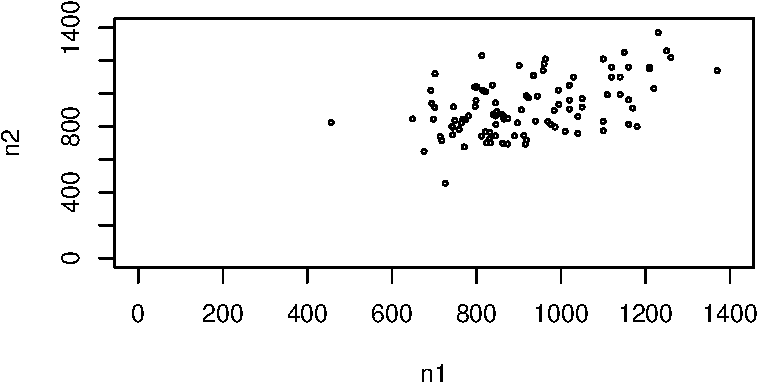
\includegraphics{Ch3_files/figure-pdf/unnamed-chunk-2-1.pdf}

}

\end{figure}

We would like to fit a straight line through that data point cloud. We
might have two motivations for doing this:

\begin{itemize}
\item
  The line might serve as nice summary of the data.
\item
  More formally, let \(C\) and \(V\) denote the current and previous
  year's measurements..Then the model
\end{itemize}

\[E(C | V) = \beta V\]

may be useful. Here the slope \(\beta\) is an unknown value to be
estimated from the data. {\marginnote{\begin{footnotesize}Readers with
some background in linear regression models should note that this
assumption of a linear trend through the origin is the only assumption
we are making here. Nothing on normal distributions
etc.\end{footnotesize}}}

\begin{tcolorbox}[enhanced jigsaw, title=\textcolor{quarto-callout-important-color}{\faExclamation}\hspace{0.5em}{Model validity}, toprule=.15mm, titlerule=0mm, colback=white, arc=.35mm, leftrule=.75mm, breakable, bottomtitle=1mm, opacityback=0, coltitle=black, colframe=quarto-callout-important-color-frame, toptitle=1mm, rightrule=.15mm, bottomrule=.15mm, colbacktitle=quarto-callout-important-color!10!white, left=2mm, opacitybacktitle=0.6]

The great statistician George Box once said, ``All models are wrong but
some are useful.'' All data scientists should keep this at the
forefronts of their minds.

\end{tcolorbox}

\hypertarget{least-squares-approach}{%
\subsection{Least squares approach}\label{least-squares-approach}}

{\marginnote{\begin{footnotesize}This too is something all data
scientists should keep at the forefronts of their minds. We are always
working with sample data, subject to intersample variations. The
quantity \(b\) is a random variable.\end{footnotesize}}} Let \(b\)
denote our estimate. How should we obtain it? We wish to estimate
\(\beta\) from our data, which we regard as a sample from the data
generating process. Denote our data by \((C_i,V_i), i = 1,...,100\).

Pretend for a moment that we don't know, say, \(C_{28}\). Using our
estimated \(\beta\), our predicted value would be \(b V_{28}\). Our
squared prediction error would then be \((C_{28} - b W_{28})^2\).

Well, we actually do know \(C_{28}\) (and the others in our data), so we
can answer the question:

In our search for a good value of \(b\), we can ask how well we would
predict our known data, using that candidate value of \(b\) in our data.
Our total squared prediction error would be

\[
\sum_{i=1}^{100} [C_{i} - b V_{i} )^2
\]

A natural choice for \(b\) would be the value that minimizes this
quantity. {\marginnote{\begin{footnotesize}Why not look at the absolute
value instead of the square? The latter makes the math flow well, as
will be seen shortly.\end{footnotesize}}}

\hypertarget{calculation}{%
\subsection{Calculation}\label{calculation}}

As noted, our choice for \(b\) will be the minimizer of

\[
\sum_{i=1}^{100} (C_{i} - b V_{i})^2
\]

This is a straightforward calculus problem. Setting

\[
0 = \frac{d}{db} \sum_{i=1}^{100} (C_{i} - b V_{i} )^2 =
-2 \sum_{i=1}^{100} (C_{i} - b V_{i}) V_i
\]

and solving \(b\), we find that

\[
b = \frac{\sum_{i=1}^n C_i V_i}{\sum_{i=1}^nV_i^2}
\]

\hypertarget{r-code}{%
\subsection{R code}\label{r-code}}

\begin{Shaded}
\begin{Highlighting}[]
\FunctionTok{lm}\NormalTok{(n2 }\SpecialCharTok{\textasciitilde{}}\NormalTok{ n1}\DecValTok{{-}1}\NormalTok{)}
\end{Highlighting}
\end{Shaded}

\begin{verbatim}

Call:
lm(formula = n2 ~ n1 - 1)

Coefficients:
  n1  
0.98  
\end{verbatim}

This says, ``Fit the model \(E(C | V) = \beta V\)\$ to the data, with
the line constrained to pass through the origin.'' The constraint is
specified by the -1 term.

We see that the estimate regression line is

\[E(C | V) = 0.98 V\]

\hypertarget{full-linear-regression-model}{%
\section{Full linear regression
model}\label{full-linear-regression-model}}

Say we do not want to constrain the model to pass the line through the
origin. Our model is then

\[E(C | V) = \beta_0 + \beta_1 V\]

where we now have two unknown parameters to be estimated.

\hypertarget{least-squares-estimation-single-predictor}{%
\subsection{Least-squares estimation, single
predictor}\label{least-squares-estimation-single-predictor}}

Our sum of squared prediction errors is now

\[
\sum_{i=1}^{100} [O_{i} - (b_0 + b_1 V_{i}) ]^2
\]

This means setting two derivatives to 0 and solving. Since the
derivatives involve two different quantities to be optimized, \(b_0\)
and \(b_1\), the derivatives are termed \emph{partial}, and the
\(\partial\) symbol is used instead of `d'.

\begin{equation}\protect\hypertarget{eq-b0}{}{
\begin{align}
0 &= 
\frac{\partial}{\partial b_0}\sum_{i=1}^{100} [C_{i} - (b_0 + b_1 V_{i })
]^2 \\
&=
-2 \sum_{i=1}^{100} [C_{i} - (b_0 + b_1 V_{i}) ] 
\end{align}
}\label{eq-b0}\end{equation}

and

\begin{equation}\protect\hypertarget{eq-b1}{}{
\begin{align}
0 &= 
\frac{\partial}{\partial b_1}\sum_{i=1}^{100} [C_{i} - (b_0 + b_1 V_{i})
]^2 \\
&=
-2 \sum_{i=1}^{100} [C_{i} - (b_0 + b_1 V_{i}) V_i] 
\end{align}
}\label{eq-b1}\end{equation}

We could then solve for the \(b_i\), but let's go straight to the
general case.

\hypertarget{least-squares-estimation-general-number-of-predictors}{%
\section{Least-squares estimation, general number of
predictors}\label{least-squares-estimation-general-number-of-predictors}}

\hypertarget{nile-example}{%
\subsection{Nile example}\label{nile-example}}

As we have seen, systems of linear equations are natural applications of
linear algebra. Equations Equation~\ref{eq-b0} and Equation~\ref{eq-b1}
can be written in matrix terms as

\[
 \left (
 \begin{array}{rr}
 \sum_{i=1}^n C_i \\
 \sum_{i=1}^n C_i V_i \\
 \end{array}
 \right ) =
 \left (
 \begin{array}{rr}
 100 & \sum_{i=1}^n V_i \\
 \sum_{i=1}^n V_i & b_1 \sum_{i=1}^n V_i^2 \\
 \end{array}
 \right ) 
 \left (
 \begin{array}{rr}
 b_0 \\
 b_1 \\
 \end{array}
 \right )
\]

Actually, that matrix equation can be derived more easily by using
matrices to begin with:

Define \(S\) and \(T\):

\[
S = 
 \left (
 \begin{array}{rr}
 C_1 \\
 C_2 \\
 ... \\
 C_{100} \\
 \end{array}
 \right )
\]

and

\[
T = 
 \left (
 \begin{array}{rr}
 V_1 \\
 V_2 \\
 ... \\
 V_{100} \\
 \end{array}
 \right )
\]

Then our linear assumption, \(E(C | V) = b_0 + b1 V\), applied to \(S\)
and \(T\), is

\[
E(S | T) =
A b
\]

where

\[
A =  
 \left (
 \begin{array}{rrrr}
 1 & V_1 \\
 1 & V_2 \\
 ... & ... \\
 1 & V_{100} \\
 \end{array}
 \right )
\]

and \(b = (b_0,b_1)'.\)

Our predicted error vector is very simply expressed:

\[
S - Ab
\]

And since for any column vector \(u\), the sum of its squared elements
is

\[
u'u
\]

our sum of squared prediction errors is

\[
(S - Ab)'(S - Ab)
\]

Now how we will minimize that matrix expression with respect to the
vector \(b\). That is the subject of the next section.

❄️ \textbf{Your Turn:} State what the matrix \(A\) would have been under
the earlier model in which the regression line is assmed to go through
the origin. And what about \((S - Ab)'(S - Ab)\) and so on? Does the
math still produce the correct answer? Note: \(b\) is now a vector of
length 1, a 1x1 matrix.

❄️ \textbf{Your Turn:} Derivative of a Show that

\[
\frac{d}{du} u'Qu = 2Qu
\]

for a constant symmetric matrix \(Q\) and a vector \(u\). (\(u'Qu\) is
called a \emph{quadratic form}.)*

\hypertarget{matrix-derivatives.}{%
\subsection{Matrix derivatives.}\label{matrix-derivatives.}}

The (column) vector of partial derivatives of a scalar quantity is
called the \emph{gradient} of that quantity. For instance, with

\[
u = 2x + 3y^2 + xy
\]

we have that its gradient is

\[
 \frac{du}{dx dy} =
 \left (
 \begin{array}{rr}
 2 + y \\
 6y + x \\
 \end{array}
 \right )
\]

With care, we can compute gradients entirely at the matrix level, using
easily derivable properties, without ever resorting to returning to the
scalar expressions. Let's apply them to the case at hand in the last
section,

\begin{equation}\protect\hypertarget{eq-rss}{}{
(S - Ab)'(S - Ab)
}\label{eq-rss}\end{equation}

\hypertarget{differentiation-purely-in-matrix-terms}{%
\subsection{Differentiation purely in matrix
terms}\label{differentiation-purely-in-matrix-terms}}

It can be shown that for a column vector \(a\),

\[
\frac{d}{da} a'a = 2a
\]

❄️ \textbf{Your Turn:} Show this. Write \(a = (a_1,...,a_k)'\) and find
the gradient ``by hand.'' Compare to \(2a\).

Equation Equation~\ref{eq-rss} is indeed of the form \(a'a\), but the
problem here is that \(a\) in turn is a function of \(b\), This calls
for the Chain Rule, which does exist at the matrix level:

For example if \(u = Mv + w\), with \(M\) and \(w\) constants (i.e.~not
functions of \(v\), then

\[
\frac{d}{dv} u'u = 2M'u
\]

With \(M = -A\) and \(w = S\), we have

\[
\frac{d}{db} [(S - Ab)'(S - Ab) = -2 A'(S - Ab)
\]

So, set

\[
0 = A'(S - Ab) = A'S - A'A b
\]

yield our minimizing \(b\):

\[
b = (A'A)^{-1} A'S
\]

providing the inverse exists (more on this in the next chapter).

Let's check this with the Nile example:

\begin{Shaded}
\begin{Highlighting}[]
\NormalTok{A }\OtherTok{\textless{}{-}} \FunctionTok{cbind}\NormalTok{(}\DecValTok{1}\NormalTok{,n1)}
\NormalTok{S }\OtherTok{\textless{}{-}}\NormalTok{ n2}
\NormalTok{Ap }\OtherTok{\textless{}{-}} \FunctionTok{t}\NormalTok{(A)}
\FunctionTok{solve}\NormalTok{(Ap }\SpecialCharTok{\%*\%}\NormalTok{ A) }\SpecialCharTok{\%*\%}\NormalTok{ Ap }\SpecialCharTok{\%*\%}\NormalTok{ S}
\end{Highlighting}
\end{Shaded}

\begin{verbatim}
          [,1]
   452.7667508
n1   0.5043159
\end{verbatim}

\begin{Shaded}
\begin{Highlighting}[]
\CommentTok{\# check via /R}
\FunctionTok{lm}\NormalTok{(n2 }\SpecialCharTok{\textasciitilde{}}\NormalTok{ n1)}
\end{Highlighting}
\end{Shaded}

\begin{verbatim}

Call:
lm(formula = n2 ~ n1)

Coefficients:
(Intercept)           n1  
   452.7668       0.5043  
\end{verbatim}

\hypertarget{the-general-case}{%
\subsection{The general case}\label{the-general-case}}

Say our data consists of \(n\) points, each of which is of length \(p\).
Write the \(j^{th}\) element of the \(i^{th}\) data point as \(X_{ij}\).
Then set

\[
A =
\left (
\begin{array}{rrrr}
1 & X_{11} & ... & X_{p1} \\
1 & X_{21} & ... & X_{p2} \\
... & ... & ... & ... \\
1 & X_{n1} & ... & X_{np} \\
\end{array}
\right )
\]

Coninue to set \(S\) to thw length-\(n\) column vector of our response
variable, and write

\[
b = (b_0,b_1,...,b_p)'
\]

Then, using the same reasoning as before, we have the minimizing value
of \(b\):

\[
b = (A'A)^{-1} A'S
\]

again providing that the inverse exists.

As an examples, let's take the \textbf{mlb1} from my
\href{https://github.com/matloff/qeML}{qeML ('Quick and Easy Machine
Learning} package. {\marginnote{\begin{footnotesize}Kindly provided by
the UCLA Dept. of Statistics\end{footnotesize}}} The data is on major
league baseball players. We will predict weight from height and age.

\begin{Shaded}
\begin{Highlighting}[]
\FunctionTok{library}\NormalTok{(qeML)}
\FunctionTok{data}\NormalTok{(mlb1)}
\FunctionTok{head}\NormalTok{(mlb1)}
\end{Highlighting}
\end{Shaded}

\begin{verbatim}
        Position Height Weight   Age
1        Catcher     74    180 22.99
2        Catcher     74    215 34.69
3        Catcher     72    210 30.78
4  First_Baseman     72    210 35.43
5  First_Baseman     73    188 35.71
6 Second_Baseman     69    176 29.39
\end{verbatim}

\begin{Shaded}
\begin{Highlighting}[]
\NormalTok{ourData }\OtherTok{\textless{}{-}} \FunctionTok{as.matrix}\NormalTok{(mlb1[,}\SpecialCharTok{{-}}\DecValTok{1}\NormalTok{]) }\CommentTok{\# must have matrix to enable \%*\%}
\FunctionTok{head}\NormalTok{(ourData)}
\end{Highlighting}
\end{Shaded}

\begin{verbatim}
  Height Weight   Age
1     74    180 22.99
2     74    215 34.69
3     72    210 30.78
4     72    210 35.43
5     73    188 35.71
6     69    176 29.39
\end{verbatim}

\begin{Shaded}
\begin{Highlighting}[]
\NormalTok{A }\OtherTok{\textless{}{-}} \FunctionTok{cbind}\NormalTok{(}\DecValTok{1}\NormalTok{,ourData[,}\FunctionTok{c}\NormalTok{(}\DecValTok{1}\NormalTok{,}\DecValTok{3}\NormalTok{)])}
\NormalTok{Ap }\OtherTok{\textless{}{-}} \FunctionTok{t}\NormalTok{(A)}
\NormalTok{S }\OtherTok{\textless{}{-}} \FunctionTok{as.vector}\NormalTok{(mlb1[,}\DecValTok{3}\NormalTok{])}
\FunctionTok{solve}\NormalTok{(Ap }\SpecialCharTok{\%*\%}\NormalTok{ A) }\SpecialCharTok{\%*\%}\NormalTok{ Ap }\SpecialCharTok{\%*\%}\NormalTok{ S}
\end{Highlighting}
\end{Shaded}

\begin{verbatim}
               [,1]
       -187.6381754
Height    4.9235994
Age       0.9115326
\end{verbatim}

\begin{Shaded}
\begin{Highlighting}[]
\CommentTok{\# check via R}
\FunctionTok{lm}\NormalTok{(Weight }\SpecialCharTok{\textasciitilde{}}\NormalTok{ .,}\AttributeTok{data=}\NormalTok{mlb1[,}\SpecialCharTok{{-}}\DecValTok{1}\NormalTok{])}
\end{Highlighting}
\end{Shaded}

\begin{verbatim}

Call:
lm(formula = Weight ~ ., data = mlb1[, -1])

Coefficients:
(Intercept)       Height          Age  
  -187.6382       4.9236       0.9115  
\end{verbatim}

\hypertarget{determinants}{%
\section{Determinants}\label{determinants}}

This is a topic that is quite straightforward and traditional, even
old-fashioned. Yet the theme of a book by Sheldon Axler,, \emph{Linear
Algebra Done Right} is that determoinants are overemphasized. He
relegates the topic to the very end of the book. Yet determinants do
appear often in applied linear algebra settings. Moreover, they will be
convenient to use in explaing very concepts in this book.

But why place the topic in this particular chapter? The answer lies in
the fact that earlier in this chapter we had the proviso ``If
\((A'A)^{-1}\) exists.'' The following property of determinants is then
relevant:

A square matrix \(G\) is invertible if and only if \(det(G) \neq 0\).

There are better ways to ascertain invertibility than this, but it is
conceptually helpful. Determinants play a similar role in the topic of
eigenveectors in Chapter 5.

\begin{Shaded}
\begin{Highlighting}[]
\FunctionTok{det}\NormalTok{(Ap }\SpecialCharTok{\%*\%}\NormalTok{ A) }
\end{Highlighting}
\end{Shaded}

\begin{verbatim}
[1] 103306202970
\end{verbatim}

Nonzero! So \((A'A)^{-1}\) does exist, confirming that our R code that
needed that property.

\hypertarget{definition}{%
\subsection{Definition}\label{definition}}

The standard definition is one of the ugliest, and least useful, in all
of mathematics. Instead we will define the term using one of the methods
for calculating determinants.

Consider an \(r \textrm{x} r\) matrix \(G\). For \(r = 2\), write \(G\)
as

\[
 G = 
 \left (
 \begin{array}{rr}
 a & b \\
 c & d  \\
 \end{array}
 \right )
 \]

and define \(\det(G)\) to be \(ad -bc\). For \(r > 2\), define
submatrices as follows.

\(G_i\) is the \((r-1) \textrm{x} (r-1)\) submatrix obtained by removing
row 1 and column \(j\) from \(G\). Then \(\det(G)\) is defined
recursively as

\[
\sum_{i=1}^r (-1)^{i+1} \det(G_i)
\]

For instance, consider

\[
 M = 
 \left (
 \begin{array}{rrr}
 5 & 1 & 0 \\
 3 & -1 & 7 \\
  0 & 1 & 1 \\
  \end{array}
 \right )
\]

The \(\det(M) = 5(-8) - 3 + 0 = -43\).

❄️ \textbf{Your Turn:} If you are familiar with recursive calls, write a
function \(\verb+dt(a)+\) to compute the determinant of a square matrix
\lstinline{a} using this scheme.

\hypertarget{properties}{%
\subsection{Properties}\label{properties}}

We state these without proof:

\begin{itemize}
\item
  \(G^{-1}\) exists if and only if \(\det(G) \neq 0\)
\item
  \(\det(GH) = \det(G) \det(H)\)
\end{itemize}

\hypertarget{update-formulas}{%
\section{Update formulas}\label{update-formulas}}

One important theme in developing prediction models (linear regression,
neural networks etc.) is that, in testing a model we fit to only a
subset of our data, then predict the remaining -- ``fresh'' -- holdout
data using the model. Or, we might do this many times, say with many
holdout sets of size 1, fitting the model on the remaining n-1 data
points each time..

This could become computationally challenging, as we would need to refit
the model each time. It would be nice if we could have an ``update''
formula that would quickly recalculate the model found on the full
dataset. In rhw case of linear models, such a formula exists, in the
Sherman-Morrison-Woodbury relation.

\bookmarksetup{startatroot}

\hypertarget{matrix-rank-and-vector-spaces-part-i}{%
\chapter{Matrix Rank, and Vector Spaces Part
I}\label{matrix-rank-and-vector-spaces-part-i}}

\newpage{}

In our computations in the latter part of the last chapter, we added a
proviso that \((A'A)^{-1}\) exists. In this chapter, we'll present a
counterexample, which will naturally lead into our covering matrix rank
and the basics of vector spaces.

\hypertarget{example-census-data}{%
\section{Example: census data}\label{example-census-data}}

This dataset is also from \textbf{qeML}. It is data for Silicon Valley
engineers in the 2000 Census. Let's focus on just a few columns.

\begin{Shaded}
\begin{Highlighting}[]
\FunctionTok{data}\NormalTok{(svcensus) }
\FunctionTok{head}\NormalTok{(svcensus) }
\end{Highlighting}
\end{Shaded}

\begin{verbatim}
       age     educ occ wageinc wkswrkd gender
1 50.30082 zzzOther 102   75000      52 female
2 41.10139 zzzOther 101   12300      20   male
3 24.67374 zzzOther 102   15400      52 female
4 50.19951 zzzOther 100       0      52   male
5 51.18112 zzzOther 100     160       1 female
6 57.70413 zzzOther 100       0       0   male
\end{verbatim}

\begin{Shaded}
\begin{Highlighting}[]
\NormalTok{svc }\OtherTok{\textless{}{-}}\NormalTok{ svcensus[,}\FunctionTok{c}\NormalTok{(}\DecValTok{1}\NormalTok{,}\DecValTok{4}\SpecialCharTok{:}\DecValTok{6}\NormalTok{)] }
\FunctionTok{head}\NormalTok{(svc) }
\end{Highlighting}
\end{Shaded}

\begin{verbatim}
       age wageinc wkswrkd gender
1 50.30082   75000      52 female
2 41.10139   12300      20   male
3 24.67374   15400      52 female
4 50.19951       0      52   male
5 51.18112     160       1 female
6 57.70413       0       0   male
\end{verbatim}

\begin{Shaded}
\begin{Highlighting}[]
\FunctionTok{lm}\NormalTok{(wageinc }\SpecialCharTok{\textasciitilde{}}\NormalTok{ .,}\AttributeTok{data=}\NormalTok{svc) }
\end{Highlighting}
\end{Shaded}

\begin{verbatim}

Call:
lm(formula = wageinc ~ ., data = svc)

Coefficients:
(Intercept)          age      wkswrkd   gendermale  
   -29384.1        496.7       1372.8      10700.8  
\end{verbatim}

So, we estimate that, other factors being equal, men about paid close to
\$11,000 more than women. This is a complex issue, but for our purposes
here, how did \textbf{gender} become \textbf{gendermale}, no explicit
mention of women?

Let's try to force the issue:

\begin{Shaded}
\begin{Highlighting}[]
\NormalTok{svc}\SpecialCharTok{$}\NormalTok{man }\OtherTok{\textless{}{-}} \FunctionTok{as.numeric}\NormalTok{(svc}\SpecialCharTok{$}\NormalTok{gender }\SpecialCharTok{==} \StringTok{\textquotesingle{}male\textquotesingle{}}\NormalTok{)}
\NormalTok{svc}\SpecialCharTok{$}\NormalTok{woman }\OtherTok{\textless{}{-}} \FunctionTok{as.numeric}\NormalTok{(svc}\SpecialCharTok{$}\NormalTok{gender }\SpecialCharTok{==} \StringTok{\textquotesingle{}female\textquotesingle{}}\NormalTok{)}
\NormalTok{svc}\SpecialCharTok{$}\NormalTok{gender }\OtherTok{\textless{}{-}} \ConstantTok{NULL}
\FunctionTok{head}\NormalTok{(svc)}
\end{Highlighting}
\end{Shaded}

\begin{verbatim}
       age wageinc wkswrkd man woman
1 50.30082   75000      52   0     1
2 41.10139   12300      20   1     0
3 24.67374   15400      52   0     1
4 50.19951       0      52   1     0
5 51.18112     160       1   0     1
6 57.70413       0       0   1     0
\end{verbatim}

\begin{Shaded}
\begin{Highlighting}[]
\FunctionTok{lm}\NormalTok{(wageinc }\SpecialCharTok{\textasciitilde{}}\NormalTok{ .,}\AttributeTok{data=}\NormalTok{svc)}
\end{Highlighting}
\end{Shaded}

\begin{verbatim}

Call:
lm(formula = wageinc ~ ., data = svc)

Coefficients:
(Intercept)          age      wkswrkd          man        woman  
   -29384.1        496.7       1372.8      10700.8           NA  
\end{verbatim}

Well, we couldn't force the issue after all. Why not? We hinted above
that \(A' A\) may not be invertible. Let's check its row-reduced form.

\begin{Shaded}
\begin{Highlighting}[]
\NormalTok{A }\OtherTok{\textless{}{-}} \FunctionTok{cbind}\NormalTok{(}\DecValTok{1}\NormalTok{,svc[,}\SpecialCharTok{{-}}\DecValTok{2}\NormalTok{])}
\NormalTok{A }\OtherTok{\textless{}{-}} \FunctionTok{as.matrix}\NormalTok{(A)}
\NormalTok{ApA }\OtherTok{\textless{}{-}} \FunctionTok{t}\NormalTok{(A) }\SpecialCharTok{\%*\%}\NormalTok{ A}
\NormalTok{ApA}
\end{Highlighting}
\end{Shaded}

\begin{verbatim}
               1        age  wkswrkd      man    woman
1        20090.0   794580.7   907240  15182.0   4908.0
age     794580.7 33956543.6 35869770 600860.8 193719.9
wkswrkd 907240.0 35869770.5 45252608 692076.0 215164.0
man      15182.0   600860.8   692076  15182.0      0.0
woman     4908.0   193719.9   215164      0.0   4908.0
\end{verbatim}

\begin{Shaded}
\begin{Highlighting}[]
\FunctionTok{library}\NormalTok{(pracma)}
\FunctionTok{rref}\NormalTok{(ApA) }
\end{Highlighting}
\end{Shaded}

\begin{verbatim}
        1 age wkswrkd man woman
1       1   0       0   0     1
age     0   1       0   0     0
wkswrkd 0   0       1   0     0
man     0   0       0   1    -1
woman   0   0       0   0     0
\end{verbatim}

Aha! The row reduction process ended prematurely. This matrix has no
inverse. We say that the matrix has \emph{rank} 4, when it needs to be
5; we also say that \(A'A\) is not of \emph{full rank}.

Recall that in the nonfull rank example we presented in the last
chapter, one row was double another. Here the sum of the last two
columns of \(A\) was equal to the first column. We say the columns are
\emph{linearly dependent}. This is the culprit in non-full rank
matrices.

In fact, not only was \(A'A\) not of full rank, but so was \(A\):

\begin{Shaded}
\begin{Highlighting}[]
\FunctionTok{qr}\NormalTok{(ApA)}\SpecialCharTok{$}\NormalTok{rank}
\end{Highlighting}
\end{Shaded}

\begin{verbatim}
[1] 4
\end{verbatim}

\begin{Shaded}
\begin{Highlighting}[]
\FunctionTok{qr}\NormalTok{(A)}\SpecialCharTok{$}\NormalTok{rank}
\end{Highlighting}
\end{Shaded}

\begin{verbatim}
[1] 4
\end{verbatim}

This is rather startling. \(A\) has over 20,000 rows --- yet only 4
linearly independent ones?{\marginnote{\begin{footnotesize}There are
many subsets of 4 rows that are linearly independent. But no sets of 5
or more are linearly independent.\end{footnotesize}}} But it follows
from this fact:

For any rxs matix \(G\), the rank of \(B\) is less than or equal to
\(\min(r,s)\).

Details to follow.

\bookmarksetup{startatroot}

\hypertarget{vector-spaces-part-ii}{%
\chapter{Vector Spaces Part II}\label{vector-spaces-part-ii}}

\newpage{}



\end{document}
